
\subsection{1.27 Сэндвичевые соединения переходных металлов с параллельными циклами (гомолигандные, гетеролигандные, многопалубные). Способы получения и условия стабильности, геометрия, электронное строение, свойства.}
\begin{figure} [H]
	\centering {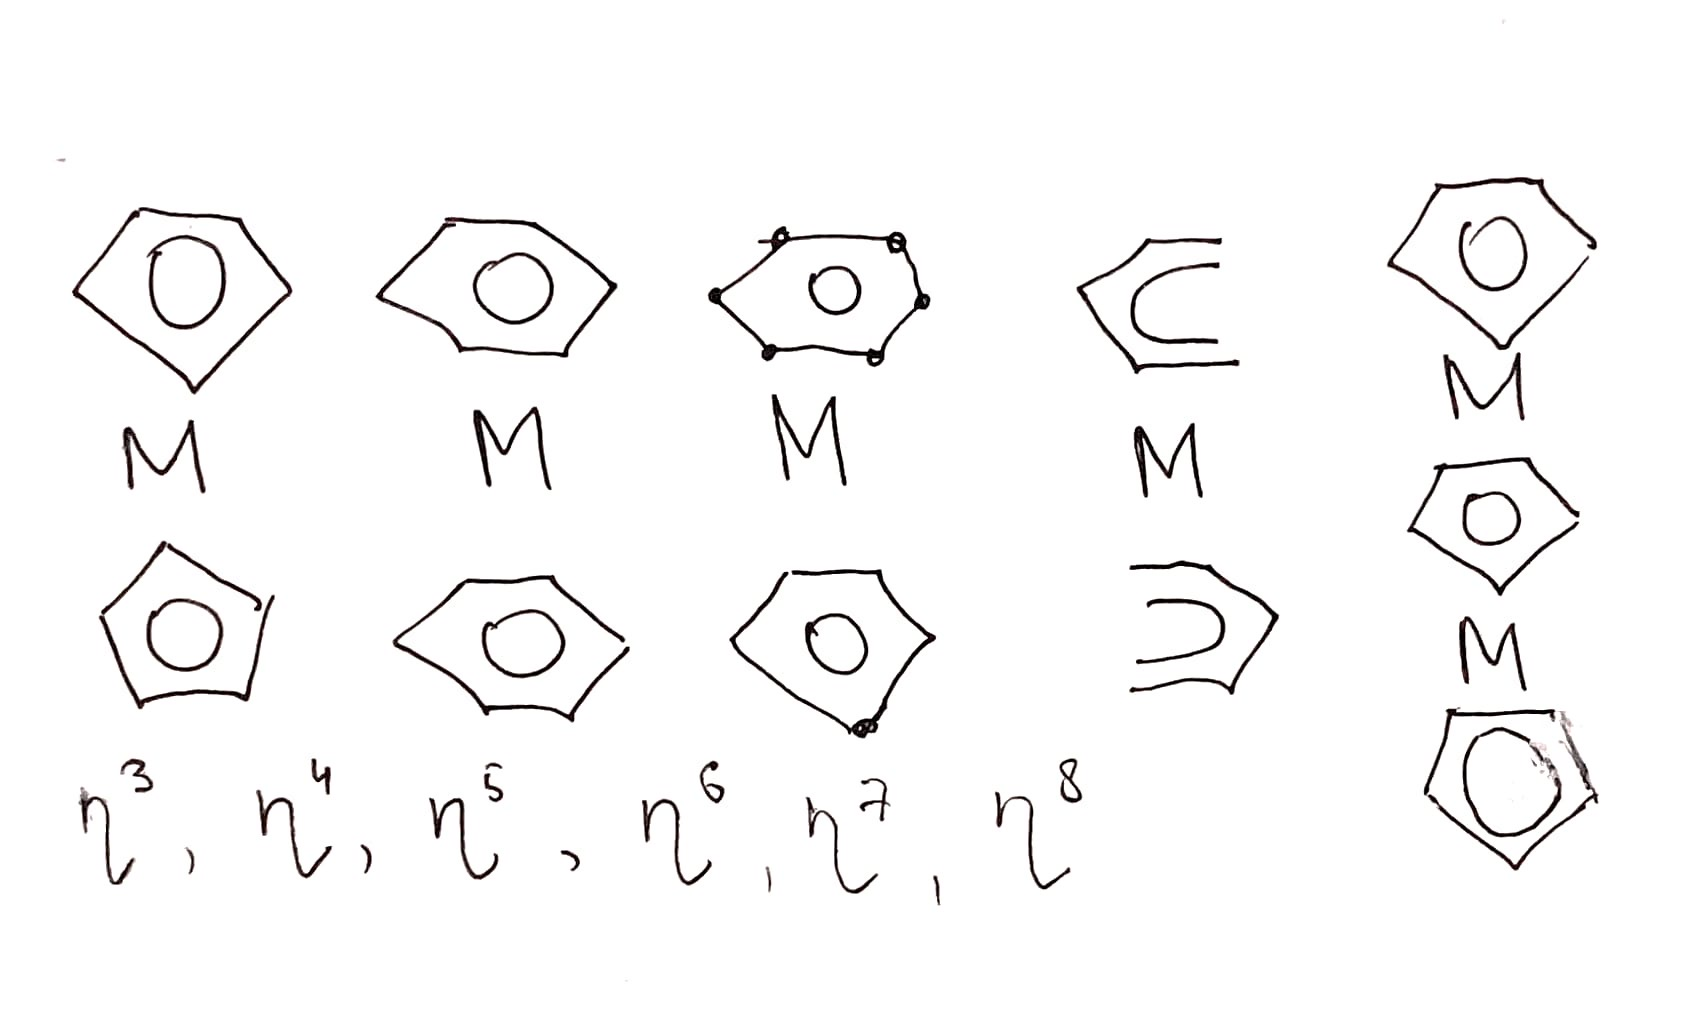
\includegraphics[scale=0.17]{xx1}}
\end{figure}
Самый устойчивый ферроцен $Cp_2Fe$ \\
Ароматичны \\
\textbf{Получение:}\\
\begin{itemize}
	\item Соль $Me$ + $Cp$-реагент
	\[
	MCl_2 + CpNa = Cp_2M \qquad (M = V, Cr, Mn, Fe, Co)
	\]
	\item Соль $Me$ + $CpH$ + осн.
	\[
	FeCl_2 + 2CpH + 2Et_2NH = Cp_2Fe + 2Et_2NH_2Cl
	\]
	\item Синтез Фишера-Хафнера
	\begin{align*}
	3CrCl_3 + 2Al + 6ArH = AlCl_3, H_2O &= \left[(ArH)_2 Cr \right]^{+} + Al^{3+} \\
	\left[(ArH)_2 Cr \right]^{+} + Na_2S_2O_4 + KOH &= (\eta^6 - ArH)_2Cr 
	\end{align*}
	\item Циклотримеризация алкинов
	\[
	(C_6H_5)_3Cr(THF)_3 + H_3C-C\equiv C-CH_3 = H_2O = (PhH)_2Cr
	\]
	\item Соконденсация из паров
	\[
	Ti\text{(г)} + 2PhH \text{(г)} = Ti(PhH)_2
	\]
	\item Получение трехпалубных 
	\begin{figure} [H]
		\centering {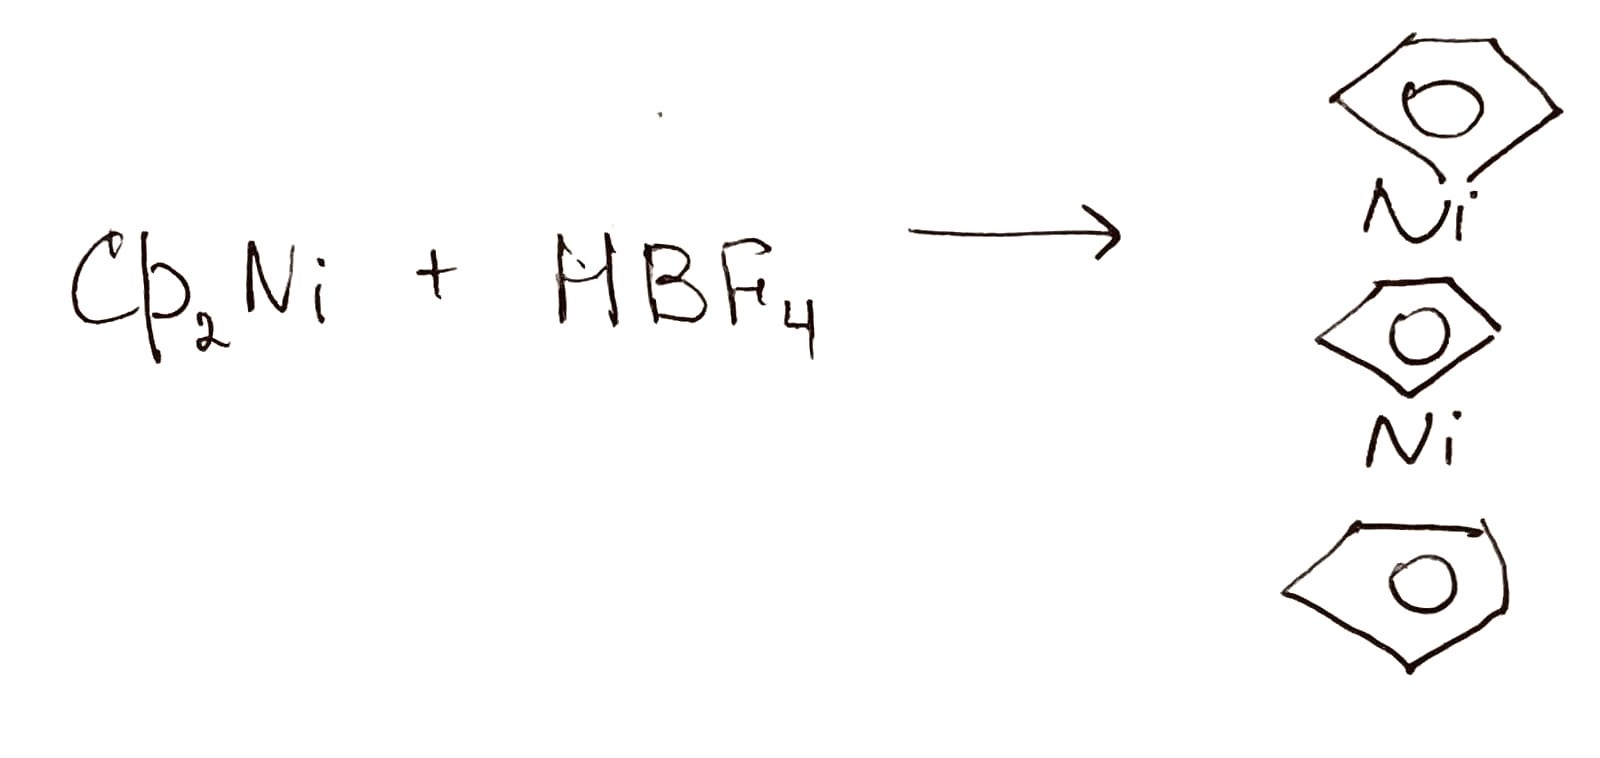
\includegraphics[scale=0.17]{xx2}}
	\end{figure}
	\item Гетеролигандные
	\begin{figure} [H]
		\centering {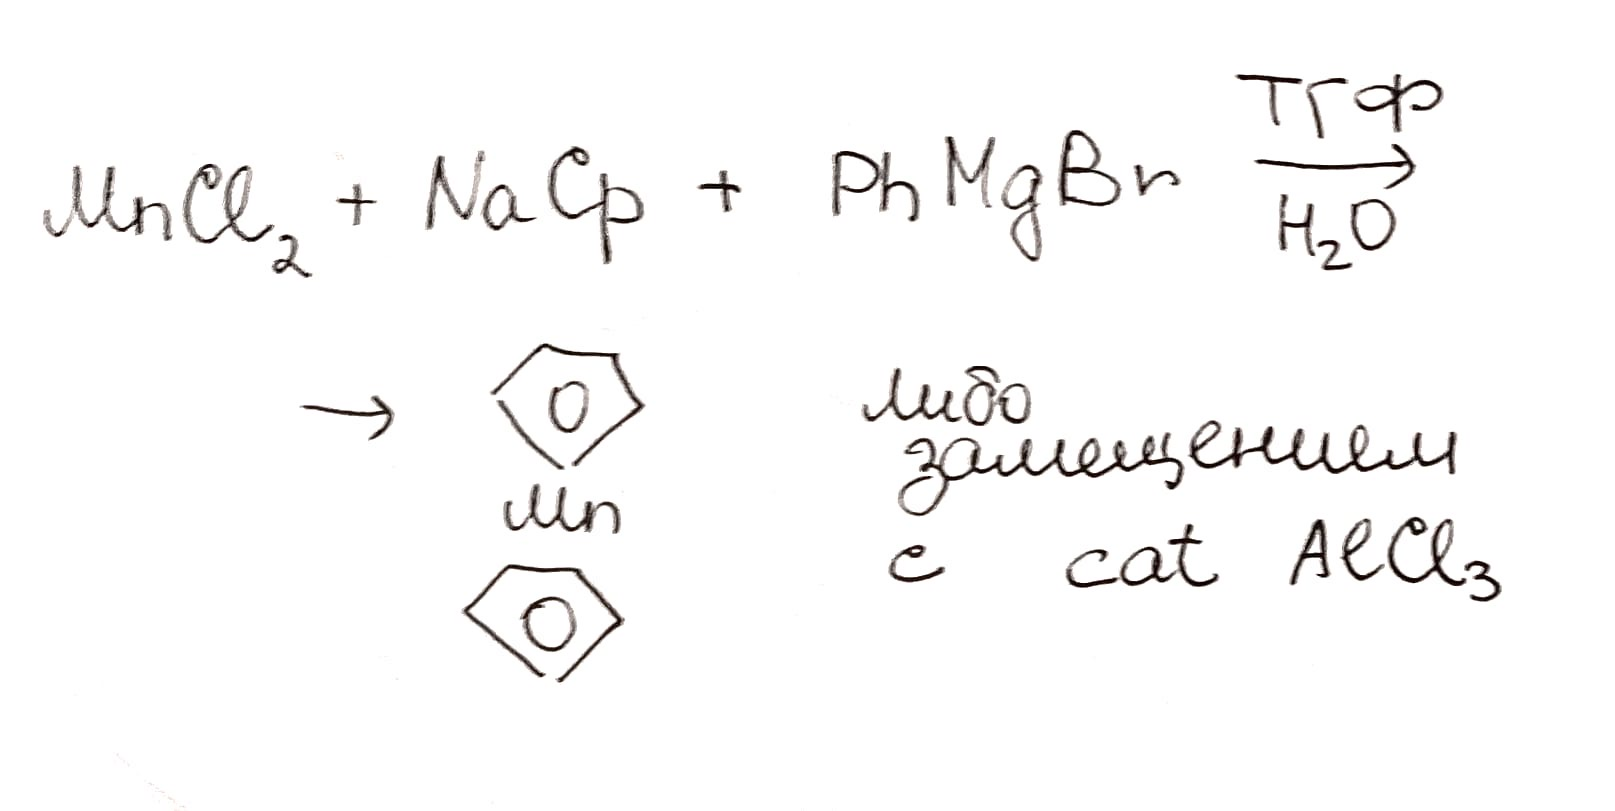
\includegraphics[scale=0.17]{xx3}}
	\end{figure}
\end{itemize}
\textbf{Условия стабильности:}\\
Правило Сиджвика не выполняется, но наиболее устойчивы те, у которых 18 электронов (нет электронов на разрыхляющих орбиталях). \\
\textbf{Геометрия:}\\
\begin{figure} [H]
	\centering {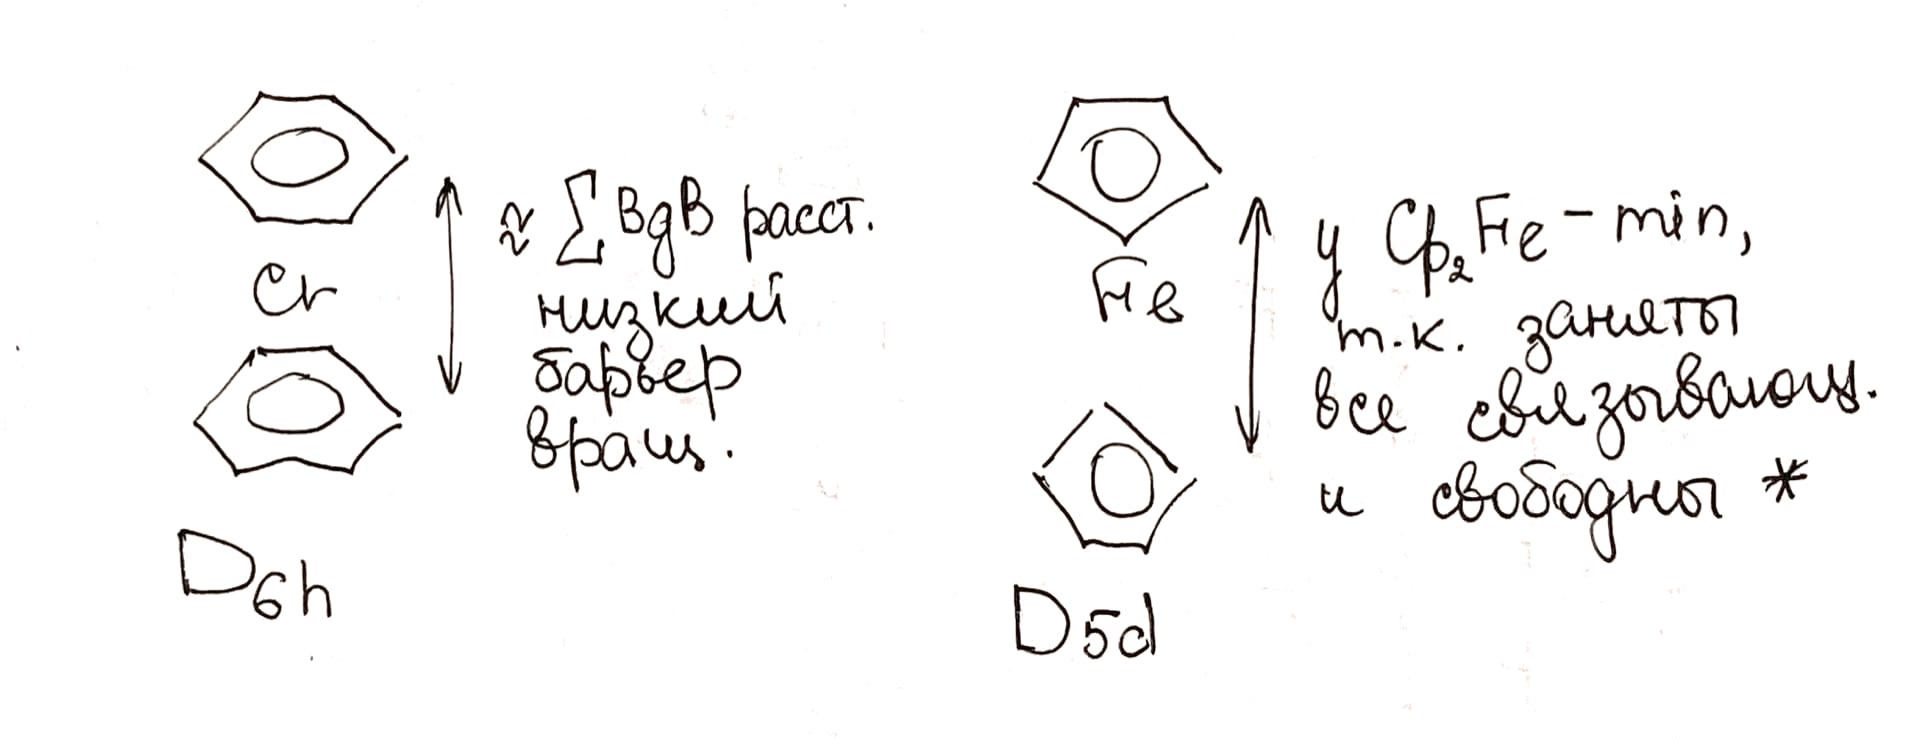
\includegraphics[scale=0.17]{xx4}}
\end{figure}
\textbf{Электронное строение (МО):}\\
\begin{figure} [H]
	\centering {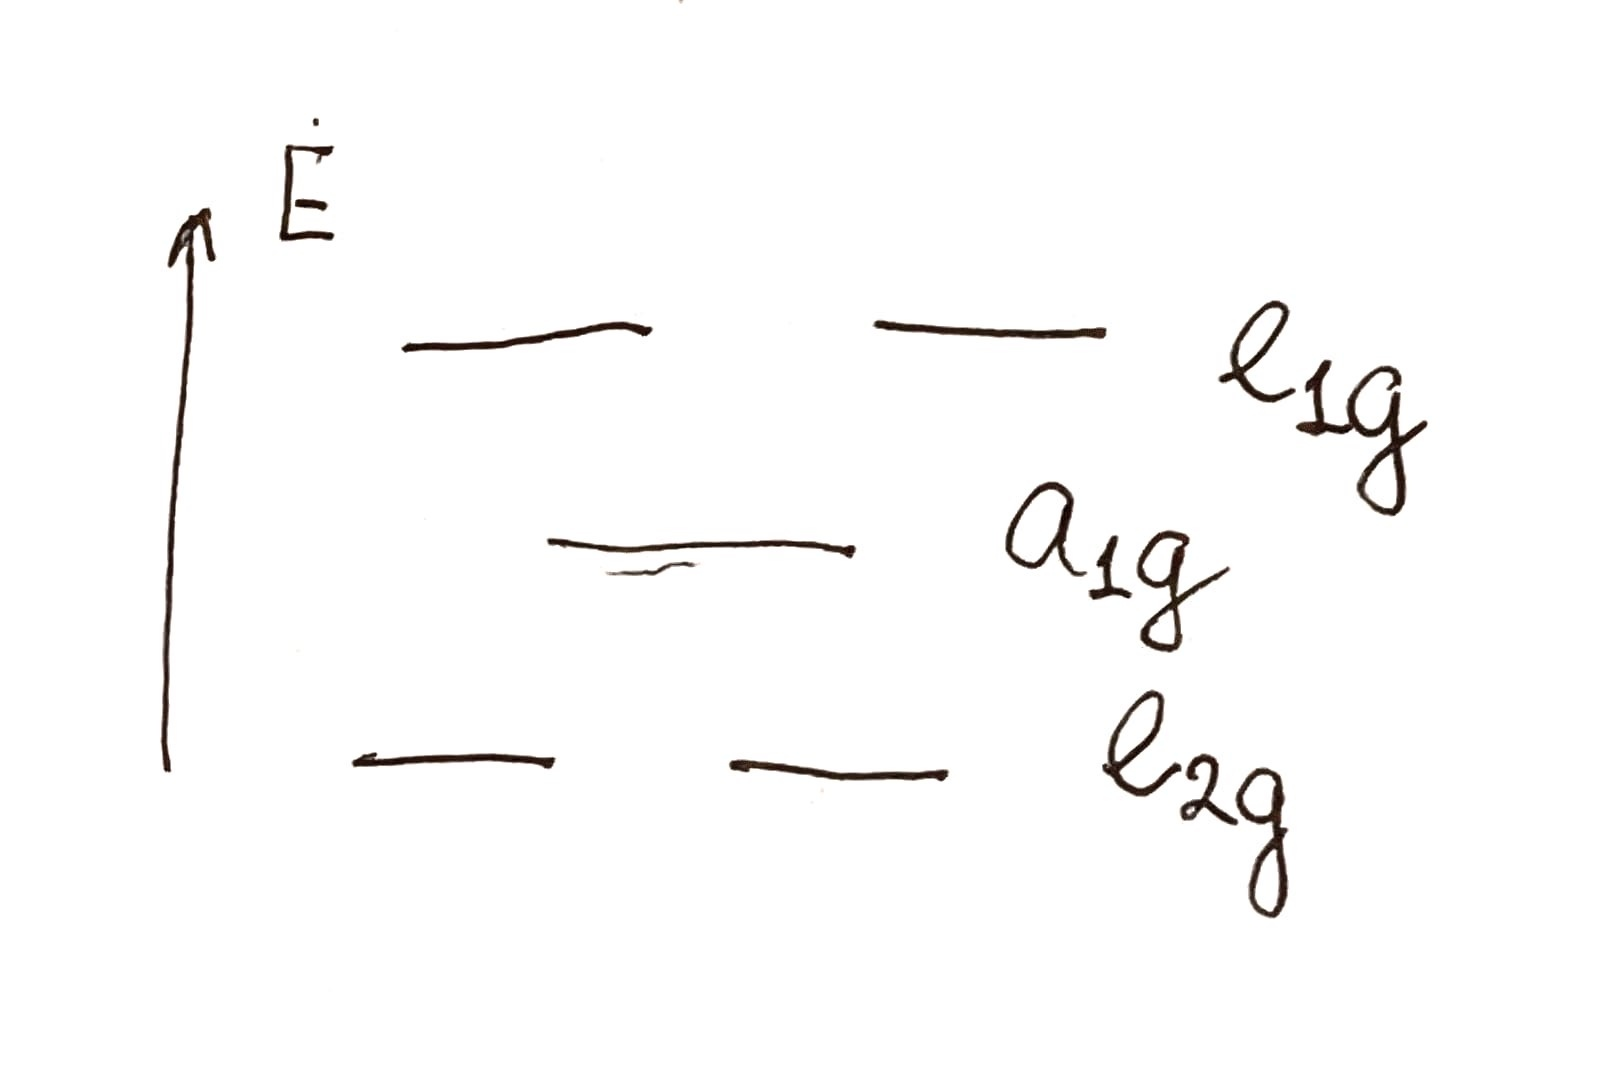
\includegraphics[scale=0.17]{xx5}}
\end{figure}
В дибензолхроме больше обратное донирование, орбитали лежат ближе по $E$ 
\textbf{Свойства:}\\
\begin{itemize}
	\item Если не 18 электронов, могут окислятся и восстанавливаться:
	\[
	Cp_2Co = -e = Cp_2Co^{+}
	\]
	\item $S_{E_{Ar}}$ (Фридель-Крафтс, металлирование)
	\item Протонирование:
	\begin{figure} [H]
		\centering {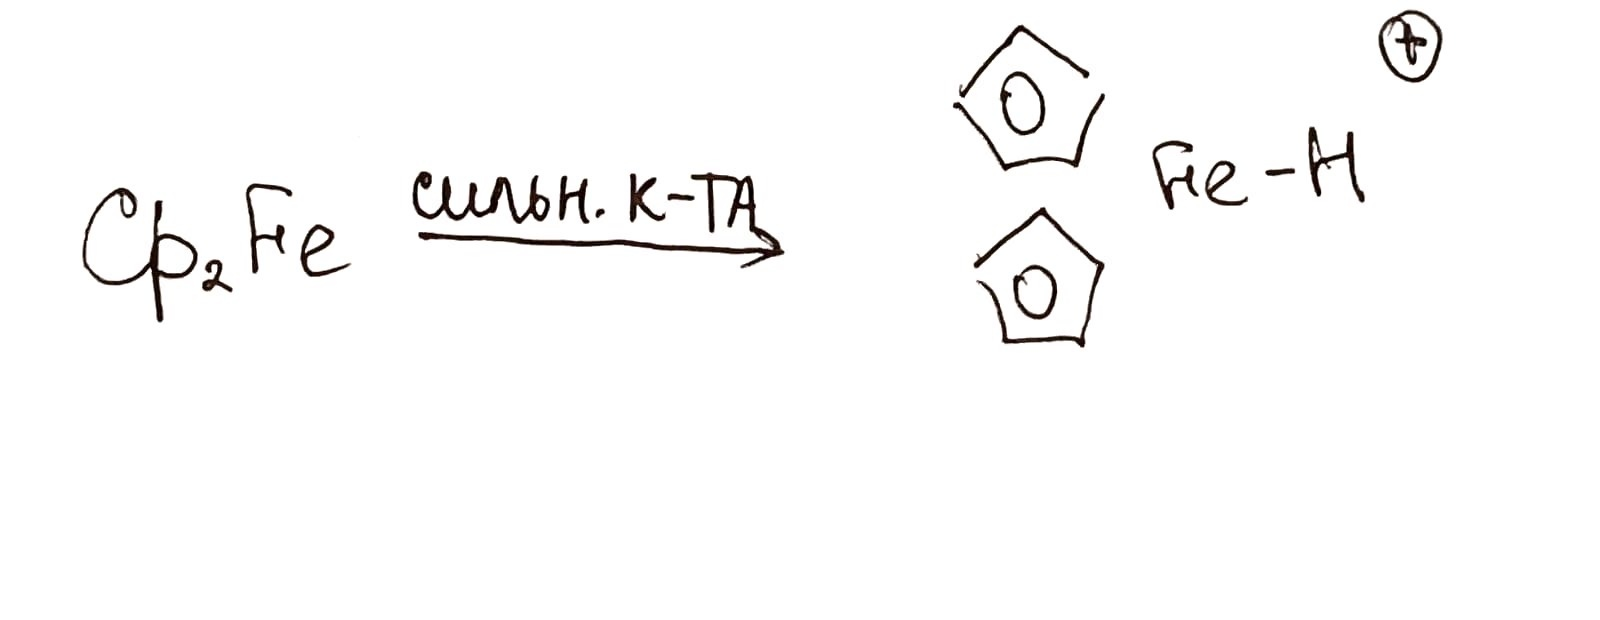
\includegraphics[scale=0.17]{xx6}}
	\end{figure}
	\item Если не 18 электронов, могут изменять гаптичность
\end{itemize}


